\chapter{Validierung des entwickelten Konzepts}
\label{ch:validierung}
Eine Validierung im Sinne der Verifizierung von Ergebnissen aus der Praxis entfällt im Rahmen dieser Arbeit. Es wird jedoch ein Simulationsmodell anhand von, in folgenden Kapiteln beschriebener, Vereinfachungen und Annäherungen aus realen Versuchsreihen an vergleichbaren Filtern aufgebaut. Das Simulationsmodell generiert hierbei Verläufe der in Kap. \ref{sec:ident_mess} ermittelten Messgrößen, mit Ausnahme der Temperatur, bis zum simulierten Versagen des Filters in Folge mechanischer Überbeanspruchung. Die so generierten Verläufe werden dann im zweiten Abschnitt der Validierung mit \ac{KNIME} untersucht, und ein \ac{ki}-Modell trainiert. Das Modell wird dann mit einem separaten Testdatensatz gespeist, um die Vorhersagegenauigkeit des Modells zu evaluieren. Das Potenzial eines derartigen prädiktiven Warnsystems werden in der Schlussbetrachtung \ref{ch:schluss} gesondert vorgestellt.
Da der Volumenstrom als Rechtecksignal simuliert wird, ist nicht von einer Verschiebung der Filtereffekte auszugehen, was sich auf die Fraktionsabscheidegrade auswirken würde, da sich somit der Filter im lt. Datenblatt empfohlenen Betriebsbereich befindet (s. Kap. \ref{sec:regelungsart}). Auf eine Simulation der Filtereffekte bie unterschiedlichen Strömugsgeschwindigkeiten wird daher verzichtet.
    \section{Erstellung Matlab/Simulink Modell}
    \label{sec:sim}
    Da im Rahmen der Arbeit keine Versuche mit Filtern vorgesehen sind, müssen für eine nachgelagerte KI-basierte Analyse die Trainingsdaten mit Hilfe einer Simulation generiert werden. Hierzu wird ein Modell in MatLab/Simulink erstellt, welches das Verhalten des Filters in Abhängigkeit von Umgebungsparametern und Volumenstrom abbildet. Da die Arbeit ein Proof-of-Concept darstellt, und nicht den Anspruch einer integrationsreifen Lösung hat, werden Annahmen für diverse Verläufe und Zusammenhänge getroffen. Der Einfluss der Temperaturen wird nicht berücksichtigt, da die Modellierung von z.B. Taupunkten und der Einfluss auf mech. Eigenschaften eine zu hohe Komplexität in Relation zum Zweck der Simulation erfordert. Die Simulation gliedert sich in das m-file, welche die Eingangsparameter und -berechnungen liefert (s. Abb. \ref{fi:mfile_parameter}), sowie die Simulation selbst (s. Abb. \ref{fi:sim_aufbau}). Da möglichst viele Reihen simuliert werden müssen, entspricht, um die Durchlaufzeit zu verringern, die Simulationszeiteinheit einer Stunde in der Realität.
    \begin{figure}[H]
        \begin{center}
            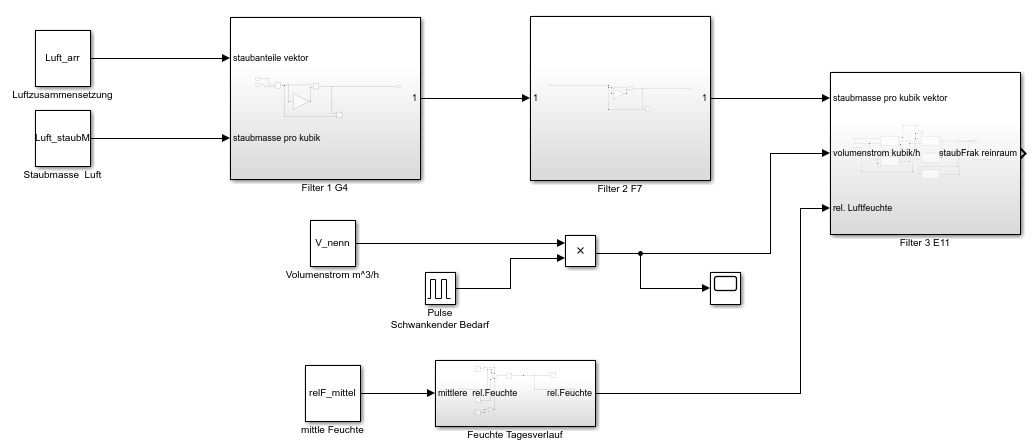
\includegraphics[width=\linewidth]{images/sim_aufbau.png}
            \caption[Aufbau Simulation]{Aufbau der Simulation}
            \label{fi:sim_aufbau}
        \end{center}
    \end{figure}
    Die Simulation ist dabei modular, dem Aufbau des Beispielsystems (s. Kap. \ref{sec:auswahl_konk}) folgend, in einzelne Filter unterteilt. Da der endständige Filter genauer untersucht werden soll, wurden die vorherigen Filter nur als Einfluss auf die Staubanteile und -masse modelliert (s. Abb. \ref{fi:sim_vorfilter}). Hierbei sind die Eingangsgrößen für beide Vorfilter die Staubmasse als Variable, sowie die Staubanteile als eindimensionaler Vektor. Durch Multiplikation miteinandern wird der Vektor zur Darstellung der Staubmasse in \si{\gram} pro \si{\cubic\meter}. Anschließend wird von den einzelnen Werten der Anteil subtrahiert, den der jeweilige Vorfilter zurückhält. Die Fraktionsabscheidegrade der Filter wurden vorher in eine Excel Datei eingetragen, welche vom m-file Skript eingelesen, und als Array behandelt werden. Hierbei ist anzumerken, das die Fraktionsabscheidegrade nicht direkt in den Datenblättern angegeben sind, sondern diese empirisch anhand von rechnerischen Abschätzungen zum Gesamtabscheidegrad bzw. Normangaben bestimmt wurden. Ausgangsgröße der Vorfiltermodule ist also ein Vektor, der die Staubmasse pro Volumen der einzelnen Staubfraktionen darstellt.
    \begin{figure}[H]
        \begin{center}
            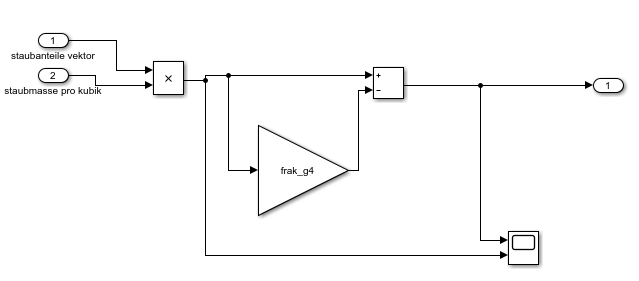
\includegraphics[width=\linewidth]{images/sim_vorfilter.png}
            \caption[Simulation der Vorfilter]{Simulation der Vorfilter}
            \label{fi:sim_vorfilter}
        \end{center}
    \end{figure}
    \subsection{Eingangsparameter}
    Die Staubzusammensetzung der Außenluft wurde nach Abb \ref{fi:staubanteile}, sowie Informationen des Umweltbundesamtes zur Staublast \cite{uba_pm10} als Array implementiert (s. Abb. \ref{fi:mfile_parameter}). Hierbei wurden jeweils Jahresmittelwerte genutzt; eine Simulation der jahreszeitlichen Schwankungen entfällt.
    \begin{figure}[H]
        \begin{center}
            \includegraphics[width=\linewidth]{images/außenluft.png}
            \caption[Außenluft Zusammensetzung]{Mittlere Staubanteile in Großstadtluft \cite{Grundlagen_Filtertechnik}}
            \label{fi:staubanteile}
        \end{center}
    \end{figure}
Da bei Fein- und Schwebstoffiltern keine Angabe zum Staubspeichervermögen gemacht werden, werden im Fall des genutzten E11-Filters Annahmen auf Grundlagen der Untersuchungen von Bergmann zu HEPA Filtern \cite{hepa} getroffen. Da sich die Umsetzung des Konzepts auf den E11-Filter konzentriert, werden analoge Berechnungen für den F7-Filter nicht durchgeführt.
Grundlage bilden dabei folgende Filterparameter \ref{fi:filterparameter}, sowie die von Bergmann ermittelten Druckdifferenzverläufe bei trockener Luft und Beaufschlagung mit Aluminiumhydroxid. Die Tabelle \ref{tab:beladungE11} zeigt hierbei die Ergebnisse der Berechnungen zur Beladung in Gramm pro \si{\square\meter} bei den untersuchten \ac{hepa} Filtern. Da die Berechnung der effektiven Fläche auch geometrische Angaben der Falten erfordern, diese aber nicht in Produktdatenblättern (s. Anhang) vermerkt sind, wird ein Faktor zur Umrechnung der Einbaufläche in effektive Fläche aufgestellt. Im Falle der von Bergmann untersuchten Filter ist die Einbaufläche \[ 18,5 in. * 23 in. = 1,285 sq. ft. \] bei einer effektiven Filterfläche von \[ 308 sq. ft. \]. Damit ergibt sich ein Faktor von \[
    240 = \frac{308 sq. ft.}{1,285 sq. ft.}
    \] für dieses Verhältnis. Da diese Filter eine Tiefe von 3 in. haben, wird der Faktor auf die Viledon Filter mit einer Faltentiefe von 100 mm angewendet. Selbstverständlich ist dieser Vergleich nicht unbedingt zulässig. Schon kleine Änderungen in der Faltengeometrie haben relativ große Auswirkungen auf die effektive Fläche, das Ziel der Arbeit ist jedoch die Vorstellung des Überwachungskonzepts, und nicht die genaue Umsetzung einer Simulation von Filtern.
    Für die Einbaugröße 610 mm x 610 mm = 0,3721 \si{\square\meter} ergibt sich hieraus mit dem Faktor 240 eine effektive Fläche von 89,3 \si{\square\meter}. Die mittlere Beladung pro \si{\square\meter} ergibt sich nach den Ergebnissen aus Tabelle \ref{tab:beladungE11} zu 14,165 \si{ \gram\per\square\metre}. Weitere geometrische Parameter wurden in Anlehnung an Bergman in metrische Einheiten umgerechnet, insofern diese nicht im Datenblatt vermerkt sind. Die entsprechenden so ermittelten Eingangsparameter wurden über das m-file implementiert (s. Abb. \ref{fi:mfile_parameter}).
\begin{figure}[H]
    \begin{center}
        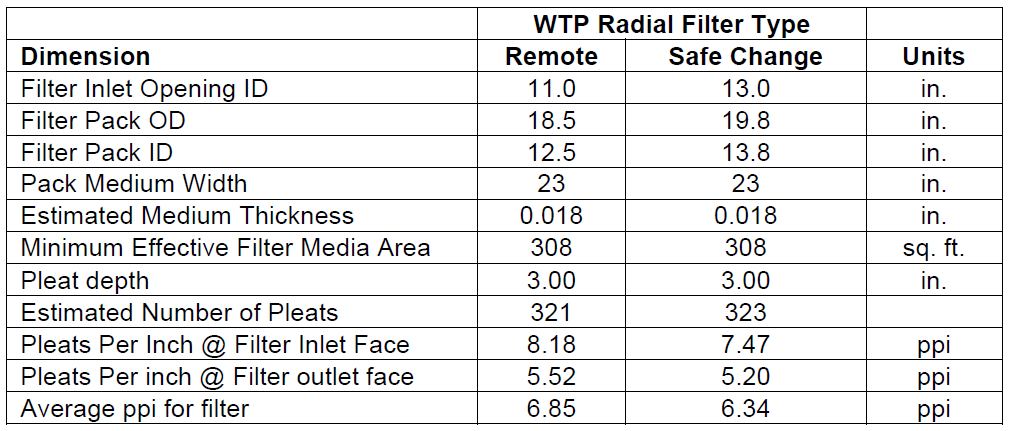
\includegraphics[width=\linewidth]{images/filter_dimensionen.png}
        \caption[Parameter HEPA Filter Bergmann]{Filterparameter untersuchter \ac{hepa} Filter von Bergmann \cite{hepa}}
        \label{fi:filterparameter}
    \end{center}
\end{figure}
\begin{table}[]
    \caption{Beladung und Druckdifferenz der Filter}
    \begin{tabular}{lllllll}
    Filter Nr. & in. WC & Druck {[}Pa{]} & Masse {[}g{]} & Fläche {[}sq.ft.{]} & Fläche{[}m2{]} & Beladung{[}g/m2{]} \\
    1          & 4      & 995            & 440           & 308                 & 28,6141        & 15,4               \\
    2          & 4      & 995            & 370           & 308                 & 28,6141        & 12,93             
    \end{tabular}
    \label{tab:beladungE11}
    \end{table}
Der Jahresmittelwert der  Staubbelastung (PM10) in Wolfsburg beträgt nach Messungen des Umweltbundesamtes 12 \si{\micro\gram\per\cubic\metre}. Wird der Massenanteil für Grobstaub nach \ref{fi:staubanteile} mit einbezogen, ergibt dies einen gesamten Massenanteil von 15,36 \si{\micro\gram\per\cubic\metre}.
    \begin{figure}[H]
        \begin{center}
            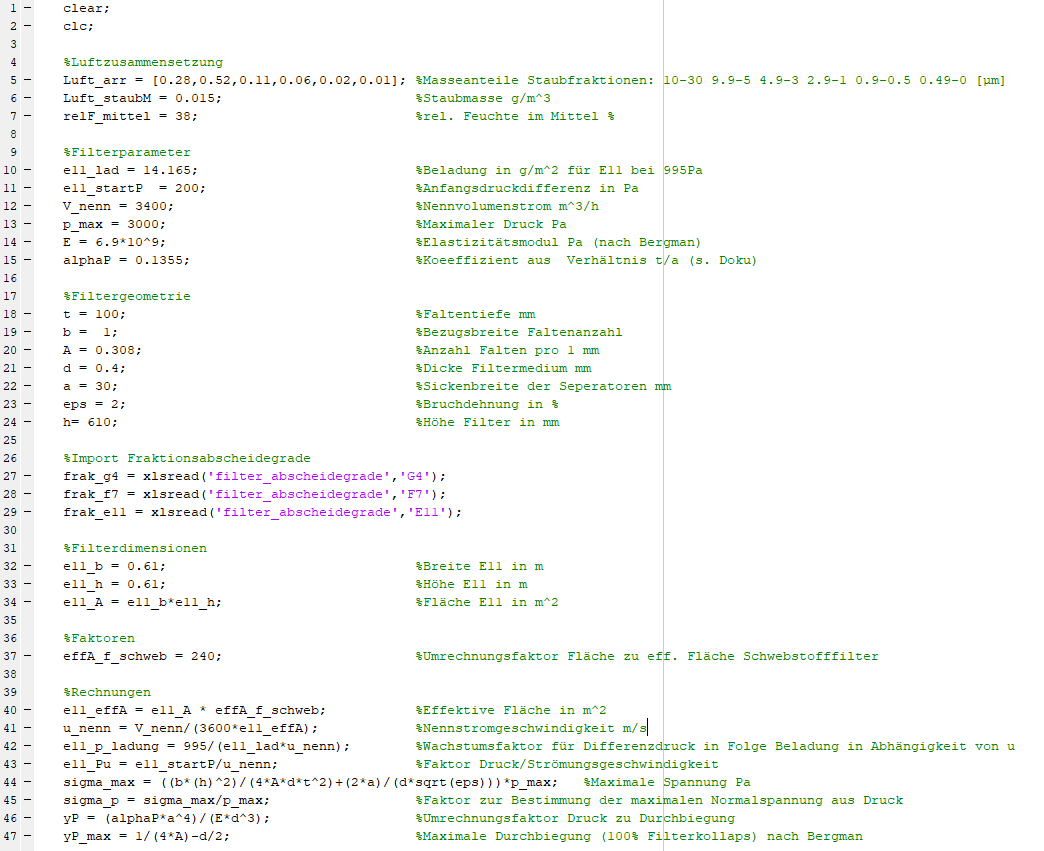
\includegraphics[width=\linewidth]{images/mfile_parameter.png}
            \caption[M-file Simulink]{Eingangsparameter und -rechnungen in m-File}
            \label{fi:mfile_parameter}
        \end{center}
    \end{figure}
    Kern der Simulation ist das Verhalten des E11 Filters (s. Abb. \ref{fi:sim_e11}). Eingangsgrößen sind hierbei der bereits erläuterte Vektor der Staubanteile, der Volumenstrom in \si{\cubic\metre\per\hour}, und die relative Luftfeuchte in \%. Essenziell für die Simulation des Filters sind zwei Subsysteme. Das Subsystem Filterleistung (s. Abb. \ref{fi:sim_filterleistung}) liefert als erste Ausgangsgröße, analog zu den Vorfiltern, die Staubanteile an der Reingasseite. Desweiteren wird die gesamte Staubmasse aus dem Eingangsvektor der Staubanteile summiert, über die Simulationszeit integriert, und mit der effektiven Filterfläche aus dem m-file zur gesamten Beladung des Filters in \si{\gram\per\square\metre} berechnet. Das zweite grundlegende Subsystem berechnet die Strömungsgeschwindigkeit aus dem Volumenstrom und der effektiven Filterfläche in \si{\metre\per\second}.
    Die weiteren Subsysteme, welche Berechnungen der mechanischen Last, Druckdifferenz usw. beinhalten, werden in den folgenden Kapiteln vorgestellt.
    \begin{figure}[H]
        \begin{center}
            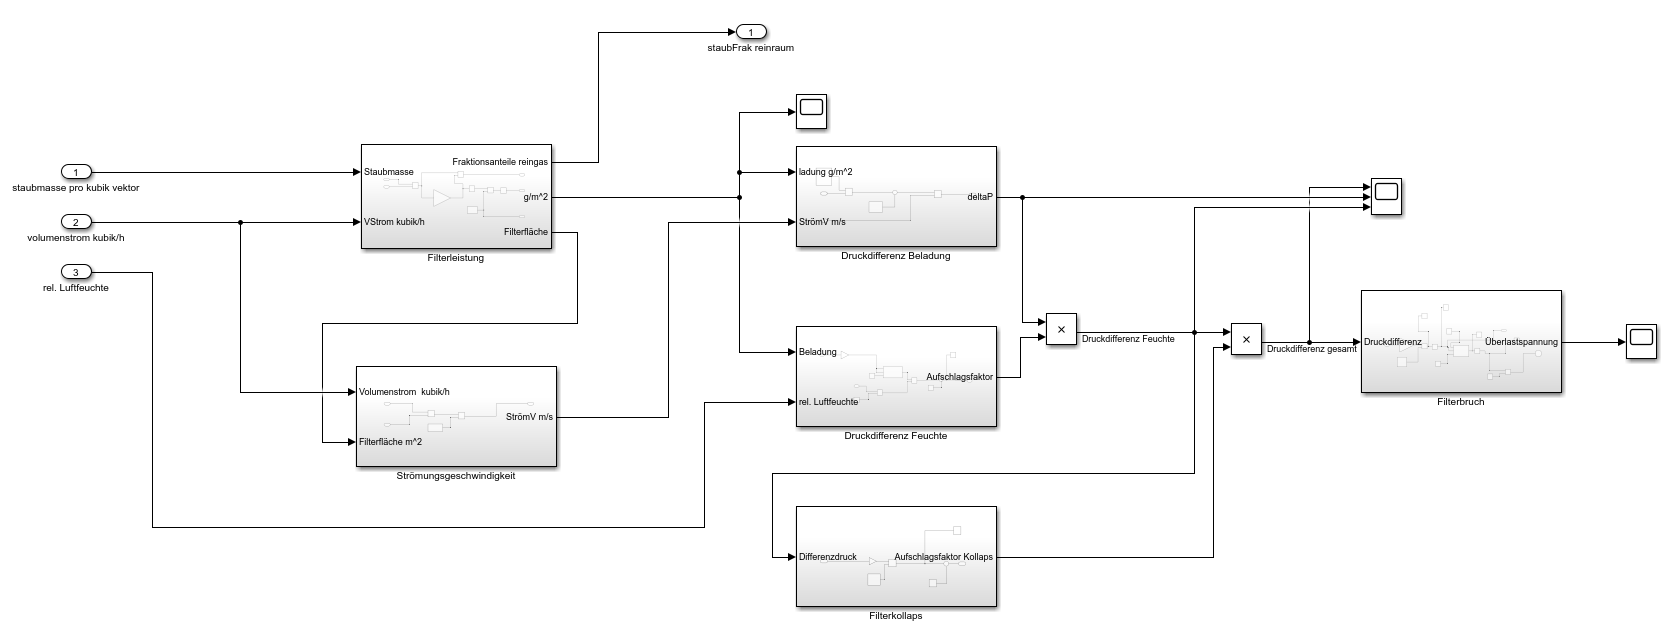
\includegraphics[width=\linewidth]{images/sim_e11.png}
            \caption[Simulation E11 Filter]{Subsystem der Simulation: endständiger E11 Filter}
            \label{fi:sim_e11}
        \end{center}
    \end{figure}
    \begin{figure}[H]
        \begin{center}
            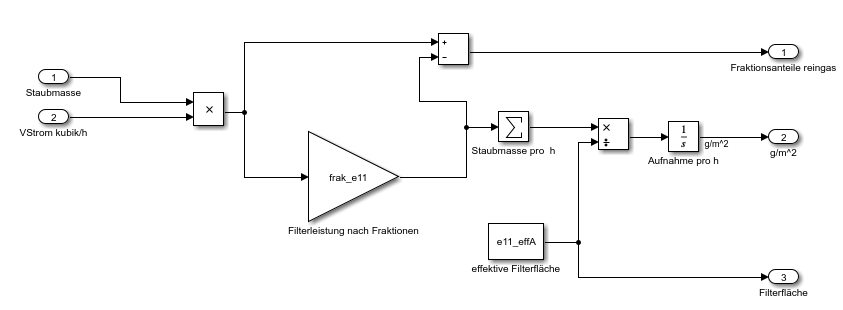
\includegraphics[width=\linewidth]{images/sim_filterleistung.png}
            \caption[Subsystem Filterleistung]{Subsystem der Simulation: Filterleistung des E11 Filters}
            \label{fi:sim_filterleistung}
        \end{center}
    \end{figure}
    \subsection{Druckverlust Beladung}
    "Der Druckverlust von Faserfiltern steigt infolge der Partikeleinlagerung im Filtermedium
mit der Zeit an. Dieses Phänomen ist bekannt, jedoch ist bis zum heutigen Wissensstand
keine gesicherte Vorausberechnung des Druckverlustanstiegs infolge der Partikelbeladung
in Faserfiltern möglich. Man ist demzufolge auf Experimente angewiesen."\cite{reinraum}
Um diesen Zusammenhang dennoch modellhaft darstellen zu können, wird vom unbeladenen Zustand bis zur empfohlenen Enddruckdifferenz bzw. Erreichen der Speicherkapazität, ein linearer Verlauf der Druckdifferenz angenommen. Die entsprechende Berechnung erfolgt im Subsystem "Druckdifferenz Beladung" (s. Abb. \ref{fi:sim_beladung}) als lineares Wachstum, wofür im m-file (s. Abb. \ref{fi:mfile_parameter}) ein Faktor für die Steigung aus Angaben des Datenblatts berechnet wird. Ausgangsgröße ist die Druckdifferenz in Pascal.
\begin{figure}[H]
    \begin{center}
        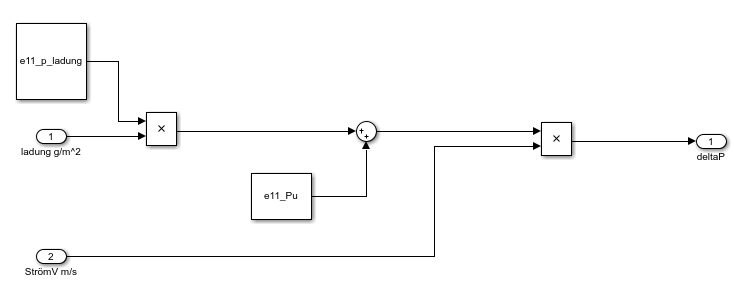
\includegraphics[width=\linewidth]{images/sim_beladung.png}
        \caption[Subsystem Druckdifferenz Beladung]{Subsystem der Simulation: Druckdifferenz durch Beladung des E11 Filters}
        \label{fi:sim_beladung}
    \end{center}
\end{figure}
\subsection{Feuchte}
Für die Modellierung des Druckverlusts in Folge hoher rel. Luftfeuchten wird die Dissertation von Ricketts' zu diesem Thema mit Bezug auf Schwebstofffiltern \cite{feuchte} zurückgegriffen. Ricketts stellt hierbei eine Grundlage zur Berechnung der steigenden Druckdifferenz in Folge von hoher Feuchte über eine bestimmte Einwirkzeit auf. Abbildung \ref{fi:parameter} verdeutlicht außerdem die Vielzahl an Einflussparametern auf den Druckwiderstand von Schwebstofffiltern, was bedingt auch auf andere Filterklassen übertragbar ist. Die Vielzahl der Parameter (s. Abb. \ref{fi:parameter}) zeigt, dass realitätsnahe Daten nahezu unmöglich mit einer Simulation generierbar sind. Die untersuchten Filter sind mit Hinblick auf die Werkstoffe der Filtermedien mit heutigen \ac{hepa} Filtern vergleichbar, da Glasfaserfiltermedien verwendet wurden. \newline
Die Sorption von Wasser durch Filter ist stark von der Staubbeladung und der Art des Staubes abhängig, da dieser Kapazitäten zur Wasseraufnahme bereitstellt. Beispielsweise wird ein Staub mit überwiegend hydrophoben Eigenschaften evtl. sogar die Aufnahme von Wasser bei gleicher Feuchte und Strömungsgeschwindigkeit verringern. \cite{feuchte} 
Die rel. Feuchte der Luft bestimmt das Gleichgewicht zwischen Adsorptions- bzw. Absorptions- und Desorptionsrate. Dies ist durch sog. Sorptionsisotherme charakterisiert, welche in der Regel empirisch ermittelt werden. In der regel stabilisiert sich die eingelagerte Wassermenge bei konstanten Parametern und ausreichend langer Einwirkzeit. Ricketts ermittelt über 70\% rel. Feuchte eine verstärkte Wassereinlagerung im Filter, und in Folge eine Änderung der Druckdifferenz (s. Abb. \ref{fi:feuchte_1}).
\begin{figure}[H]
    \begin{center}
        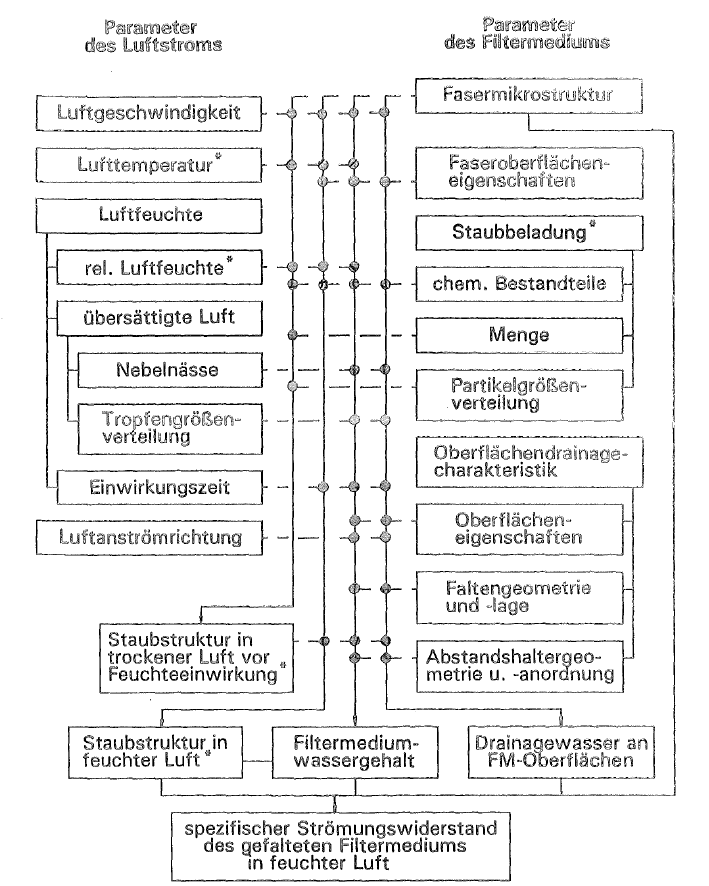
\includegraphics[width=1.1\linewidth]{images/parameter.png}
        \caption[Einflussparameter Ricketts]{Luftstrom- und Filtermediumparameter mit Einfluss auf den Strömungswiderstand von Schwebstofffiltern nach Ricketts \cite{feuchte}}
        \label{fi:parameter}
    \end{center}
\end{figure}
\begin{figure}[H]
    \begin{center}
        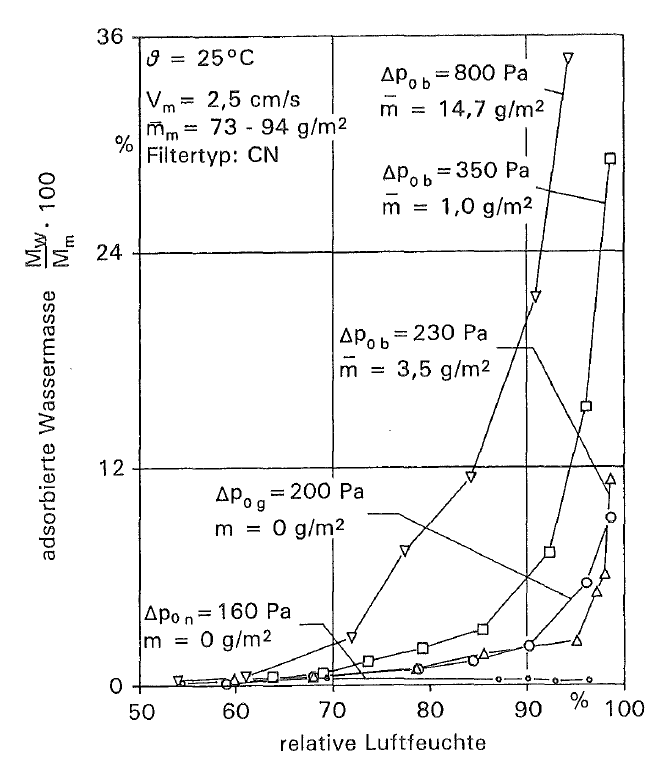
\includegraphics[width=0.95\linewidth]{images/feuchte_1.png}
        \caption[Materialfeuchte rel. Luftfeuchte]{Absorptionstherme von Filterproben in verschiedenen Zuständen \cite{feuchte} S.55}
        \label{fi:feuchte_1}
    \end{center}
\end{figure}
   Der Einfluss der Materialfeuchte auf die Druckdifferenz ist ein zeitabhängiger Vorgang und der Verlauf der Druckdifferenz ähnelt hierbei einer Sättigungskurve auf den etwa dreifachen Wert (s. Abb. \ref{fi:feuchte_2}). Eine Modellierung der Zeitabhängigkeit der Feuchteaufnahme und Druckdifferenz in der Simulation wäre wünschenswert, trägt aber nicht zum Ziel der Arbeit bei. Die Verläufe müssen in jedem Fall empirisch an Filterproben mit unterschiedlichem Beladungszustand und Feuchte ermittelt werden, um eine genaue Modellerierung zu gewährleisten. Wurden diese Verläufe erfasst, bestenfalls unter Verwendung von \ac{doe} Methoden, liegt bereits eine extensive Datenbasis vor, für die sich eine KI basierte Analyse anbietet. 
   \begin{figure}[H]
    \begin{center}
        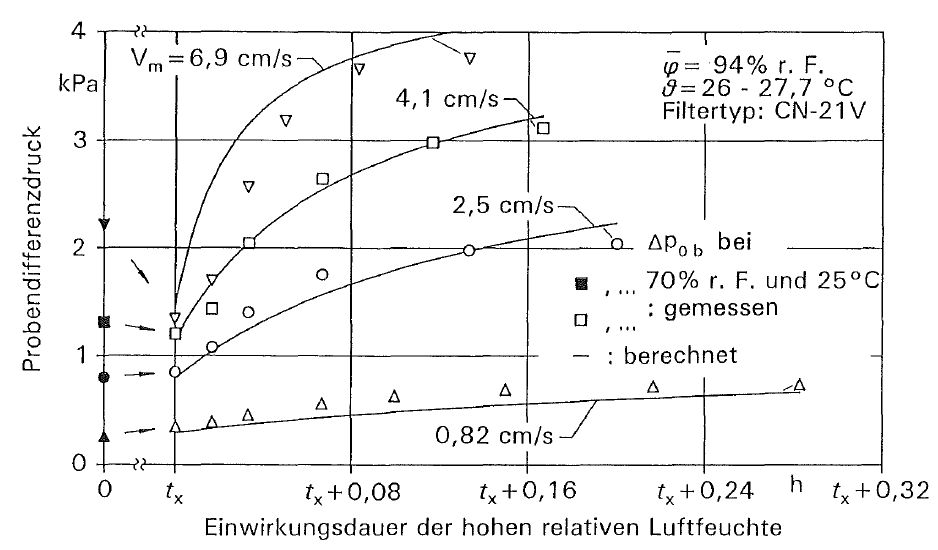
\includegraphics[width=0.9\linewidth]{images/feuchte_2.png}
        \caption[Differenzdruckverläufe Filterproben]{Differenzdruckverläufe der Proben bei unterschiedlichen Anströmgeschwindigkeiten \cite{feuchte} S.72}
        \label{fi:feuchte_2}
    \end{center}
\end{figure}
    Im Modul "Druckdifferenz Feuchte" wird (s. Abb. \ref{fi:sim_feuchte}) zunächst der Feuchtewert von Prozent in einen Dezimalwert umgerechnet. Der Switch-Block gibt den Feuchtewert nur überhalb 70\% weiter. Die Einwirkzeit wird bei erstellten Modul nicht berücksichtigt. Jedoch wird der Wert der Feuchte mit der Beladung verrechnet und ein Aufschlagsfaktor gebildet, so dass bei 100\% rel. Feuchte und 15 \si{\gram\per\square\metre} (nachträglich in Sim. korrigiert) eine Verdopplung der Druckdifferenz eintritt. Dieser Faktor wurde auf Grundlage der erreichten Druckdifferenzen von 800 bzw. 350 Pascal der mit 14,7 bzw. 1 \si{\gram\per\square\metre} beladenen Proben aus Abb. \ref{fi:feuchte_1} approximiert.
    \begin{figure}[H]
        \begin{center}
            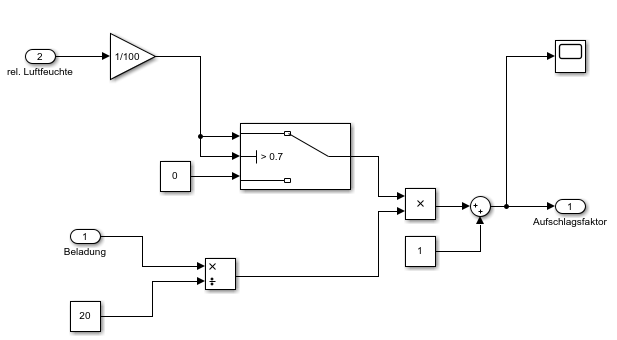
\includegraphics[width=0.9\linewidth]{images/sim_feuchte.png}
            \caption[Subsystem Druckdifferenz Feuchte]{Subsystem der Simulation: Druckdifferenz durch Feuchteeinwirkung auf den E11 Filter}
            \label{fi:sim_feuchte}
        \end{center}
    \end{figure}
\begin{figure}
    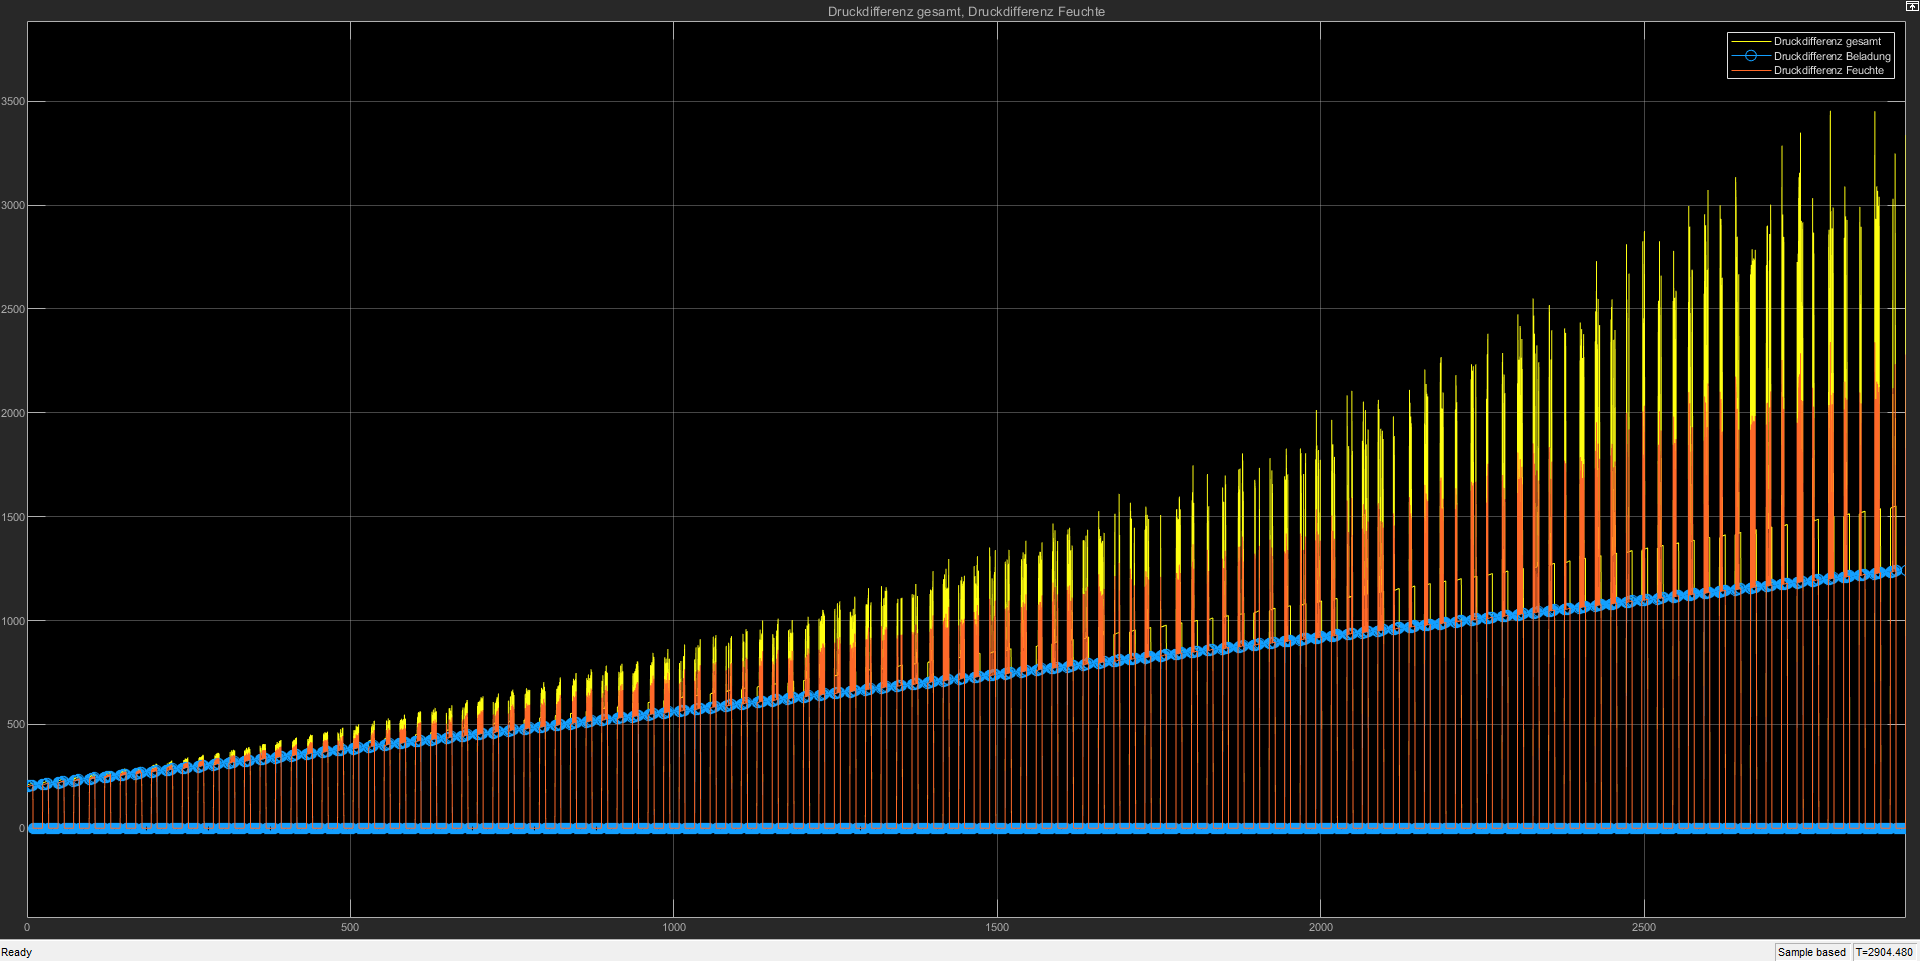
\includegraphics[height=0.85\textwidth,angle=90,origin=c]{images/sim_verlauf_druck.png}
    \caption[Simulierter Verlauf der Druckdifferenz am E11 Filter]{Simulierter Verlauf der Druckdifferenz am E11 Filter. gelb: $\Delta p_{gesamt}$, blau: $\Delta p_{Beladung}$,orange: blau: $\Delta p_{Feuchte}$}
    \label{fi:sim_verlauf_druck}
    \end{figure}
    \ \newpage
    \subsection{Simulation Filterkollaps und Versagen}
    In Anlehnung an die Berechnungen von Bergman \cite{hepa} wurde die maximale Durchbiegung ($y_{pmax}$) im m-File (s. Abb. \ref{fi:mfile_parameter}) aus den abgeschätzten geometrischen Eigenschaften des Filters bestimmt. Bei der betrachteten Schadensart handelt es sich um eine Kombination der in Abb. \ref{fig:schadensarten} vorgestellten Schadensarten an den Falten und Bersten des Mediums, in Kombination mit Filterkollaps. Die anderen Schadensarten wurden überschlägig mit den von Rüdinger \cite{rudinger} ermittelten Formeln überprüft. Da keine Informationen zur Verklebung mit dem Rahmen bekannt sind, können diese nicht einbezogen werden. Die anderen Lasten erreichten bei $ \Delta p = \SI{3}{\kilo\pascal}$ nur etwa ein Zehntel der später ermittelten zulässigen Spannung mit den von Rüdinger aufgestellten Formeln.
    Entscheidend für die Durchbiegung sind das Elastizitätsmodul \ac{Eps}, die Druckdifferenz \ac{p}, der Faktor $\alpha$ und die geometrischen Eigenschaften. 
    \ac{Eps} wurde nach Bergman zu \SI{6,9e9}{\pascal} bestimmt. 
    Da keine Werkstoffeigenschaften für den untersuchten Filter ermittelbar waren, und dieser Wert mit den Angaben von Herstellern für Glasfaserpapiere in etwa übereinstimmt, wurde dieser übernommen. 
    Der Wert von 0,1355 für $\alpha$ wurde aus der Tabelle von Bergman hierfür mit linearer Regression errechnet. Die so ermittelten Werte wurden im m-file eingespeist, und das Modul (s. Abb. \ref{fi:sim_kollaps}) berechnet hieraus, analog zum Feuchte Modul, einen Aufschlagsfaktor für die Druckdifferenz. 
    Hierbei ist anzumerken, dass bei halber Durchbiegung eine Halbierung der Filterfläche, und somit eine Verdopplung der Druckdifferenz eintritt. 
    Eigentlich wäre der Filterkollaps bzw. der Verlauf der Druckdifferenz von einer gegenseitigen Rückkopplung betroffen. 
    Die Modellierung eben dieser entfällt bei der Simulation auf Grund der hohen Komplexität der physikalischen Gleichgewichtsvorgänge bei diesem Ereignis.
    \begin{figure}[H]
        \begin{center}
            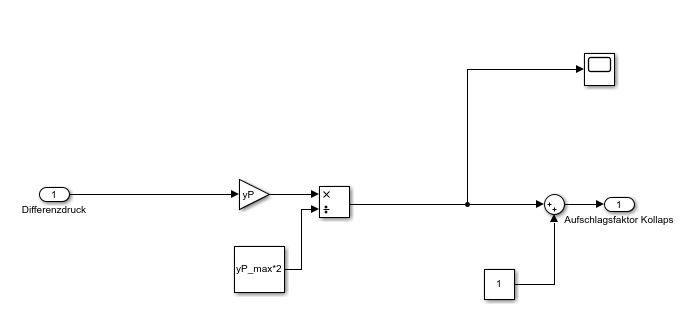
\includegraphics[width=\linewidth]{images/sim_kollaps.png}
            \caption[Subsystem Filterkollaps]{Subsystem der Simulation: Filterkollaps durch Verformung des Filtermediums}
            \label{fi:sim_kollaps}
        \end{center}
    \end{figure}
    Das Filterversagen wird nun im Subsystem Filterbruch (s. Abb. \ref{fi:sim_filterbruch}) modelliert. Hierzu wird zunächst aus der, im Datenblatt angegebenen, maximalen Druckdifferenz ein Wert für die maximal zulässige Spannung $\sigma_{max}$ im m-file (s. Abb. \ref{fi:mfile_parameter}) berechnet. Dies erfolgt nach Rüdinger's Formel zur Abschätzung der maximalen Normalspannung im Filtermedium unter Drucklast \cite{rudinger} (zur Bezeichnung der Variablen s. m-file \ref{fi:mfile_parameter})
    \[
    \sigma_{max} = (\frac{b*h^2}{4*A*d*t^2}+\frac{2*a}{d*\sqrt{\epsilon}})*\Delta p
    \]
    Aus dieser Formel wird ebenfalls ein Umrechnungsfaktor $sigma_p$ im m-file berechnet, welcher zur Konvertierung von Druckdifferenz in Normalspannung genutzt wird. Von der so errechneten Spannung wird zur Laufzeit $\sigma_{max}$ subtrahiert, und das Ergebnis mit einem Saturation Block auf positive Ergebnisse begrenzt. Der somit erreichte Verlauf ist in Abbildung \ref{fi:sim_verlauf_uberlast} zu sehen. Der Switch Block nimmt nun nur dann eine Möglichkeit zur Schadensbildung an, wenn $\sigma_{max}$ um \SI{1}{\kilo\pascal} überschritten wird. Hierzu wird, im Falle einer Überschreitung, eine Zufallsvariable zwischen 1 und 100 geschaltet, um den statistischen Charakter von Materialversagen darzustellen. Um durch Zufallsverläufe hervorgerufene Spitzen im Zeitbereich unter einer Minute auszugleichen wird diese Schadenswahrscheinlichkeit über die Simulationszeit integriert, und die Simulation bei Überschreiten der so kumulierten Schadenswahrscheinlichkeit von 100\% gestoppt. Dies kommt dem eintreten eines Filterbruchs gleich.
    Welche Größe bzw. ob die erreichte Lebensdauer Zielgröße für die KI-basierte Analyse wird, wird in Kapitel \ref{sec:knime} evaluiert.
    \begin{figure}[H]
        \begin{center}
            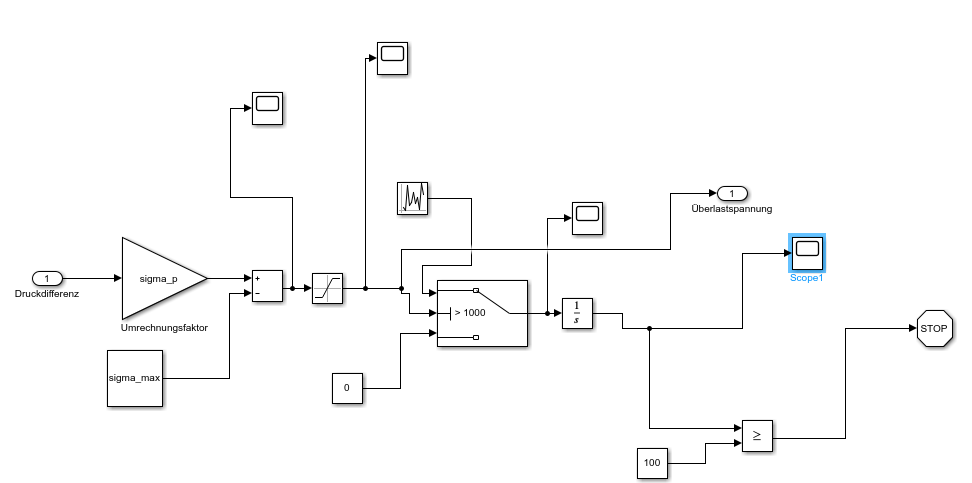
\includegraphics[width=\linewidth]{images/sim_filterbruch.png}
            \caption[Subsystem Filterbruch]{Subsystem der Simulation: Filterbruch in Folge von Überschreiten der max. zulässigen Spannung}
            \label{fi:sim_filterbruch}
        \end{center}
    \end{figure}
    \begin{figure}
        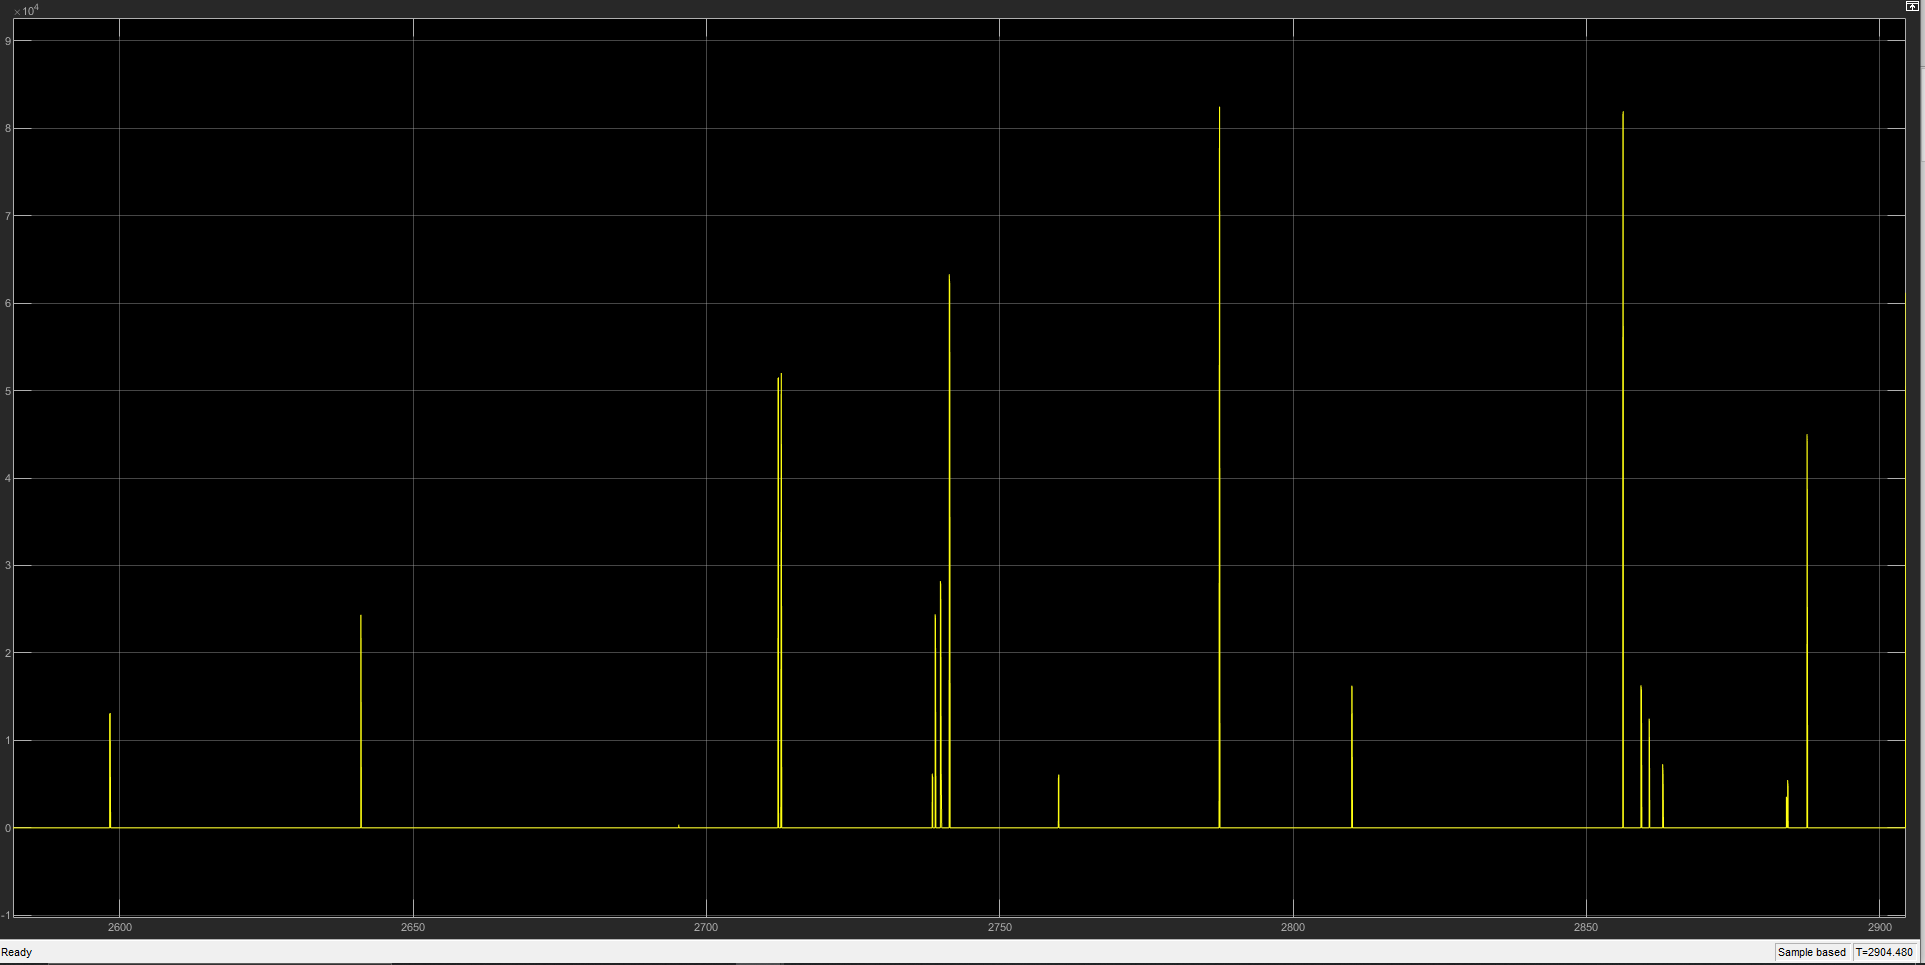
\includegraphics[height=0.85\textwidth,angle=90,origin=c]{images/sim_verlauf_uberlast.png}
        \caption[Simulierter Verlauf der Überlastspannung am E11 Filter]{Simulierter Verlauf der Überlastspannung (in Pa) am E11 Filter.}
        \label{fi:sim_verlauf_uberlast}
        \end{figure}
        \ \newpage
    \subsection{Simulation Einführung von Zufall und Varianz in Feuchte und Volumenstrom}
    Da der Volumenstrom belegungsgesteuert ist, wird ein Pulsgenerator Block mit rechteckigem Ausgangssignal von 0 bis 1 genutzt. Dieser modelliert eine Nutzung der Räumlichkeiten von $9+(\frac{10n}{48})$ Stunden pro Tag (s. Abb. \ref{fi:sim_aufbau}). Um die jahres- und tageszeitlichen Schwankungen zu modellieren werden im Subsystem Feuchte Tagesverlauf zwei Sinuswellen Generatoren eingesetzt. Die Amplituden orientieren sich hierbei an gemessenen Jahres- und Tagesverläufen des deutschen Wetterdienstes, während die Frequenzen an die jeweilige Zeiteinheit mit Berücksichtigung der Simulationszeiteinheit von einer Stunde festgelegt wurden. Die simulierten Feuchtewerte schwanken somit um einen Jahresmittelwert der Feuchte für einen fiktiven Standort (Raum Wolfsburg bzw. Braunschweig wurde recherchiert), welcher im m-file hinterlegt wurde, und in der Simulation mit $\frac{n}{10}$ addiert wird. Zusätzlich wurde eine Zufallsvariablen eingeführt, um durchs Wetter hervorgerufene Schwankungen der Feuchte wenigstens annähernd abzubilden. Der erzeugte Verlauf ist beispielhaft an einem Durchlauf in Abb. \ref{fi:sim_verlauf_feuchte} zu sehen.
    \begin{figure}[H]
        \begin{center}
            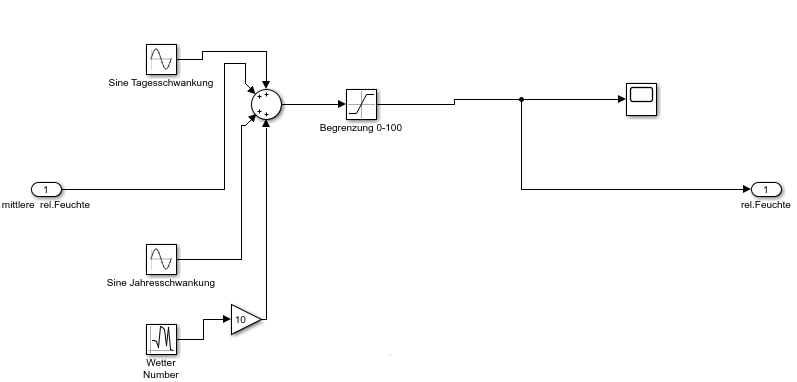
\includegraphics[width=0.8\linewidth]{images/sim_feuchteschwank.png}
            \caption[Subsystem Feuchte Tagesverlauf]{Subsystem der Simulation: Modellierung der Schwankungen der rel. Feuchte}
            \label{fi:sim_feuchteschwank}
        \end{center}
    \end{figure}
\begin{figure}
    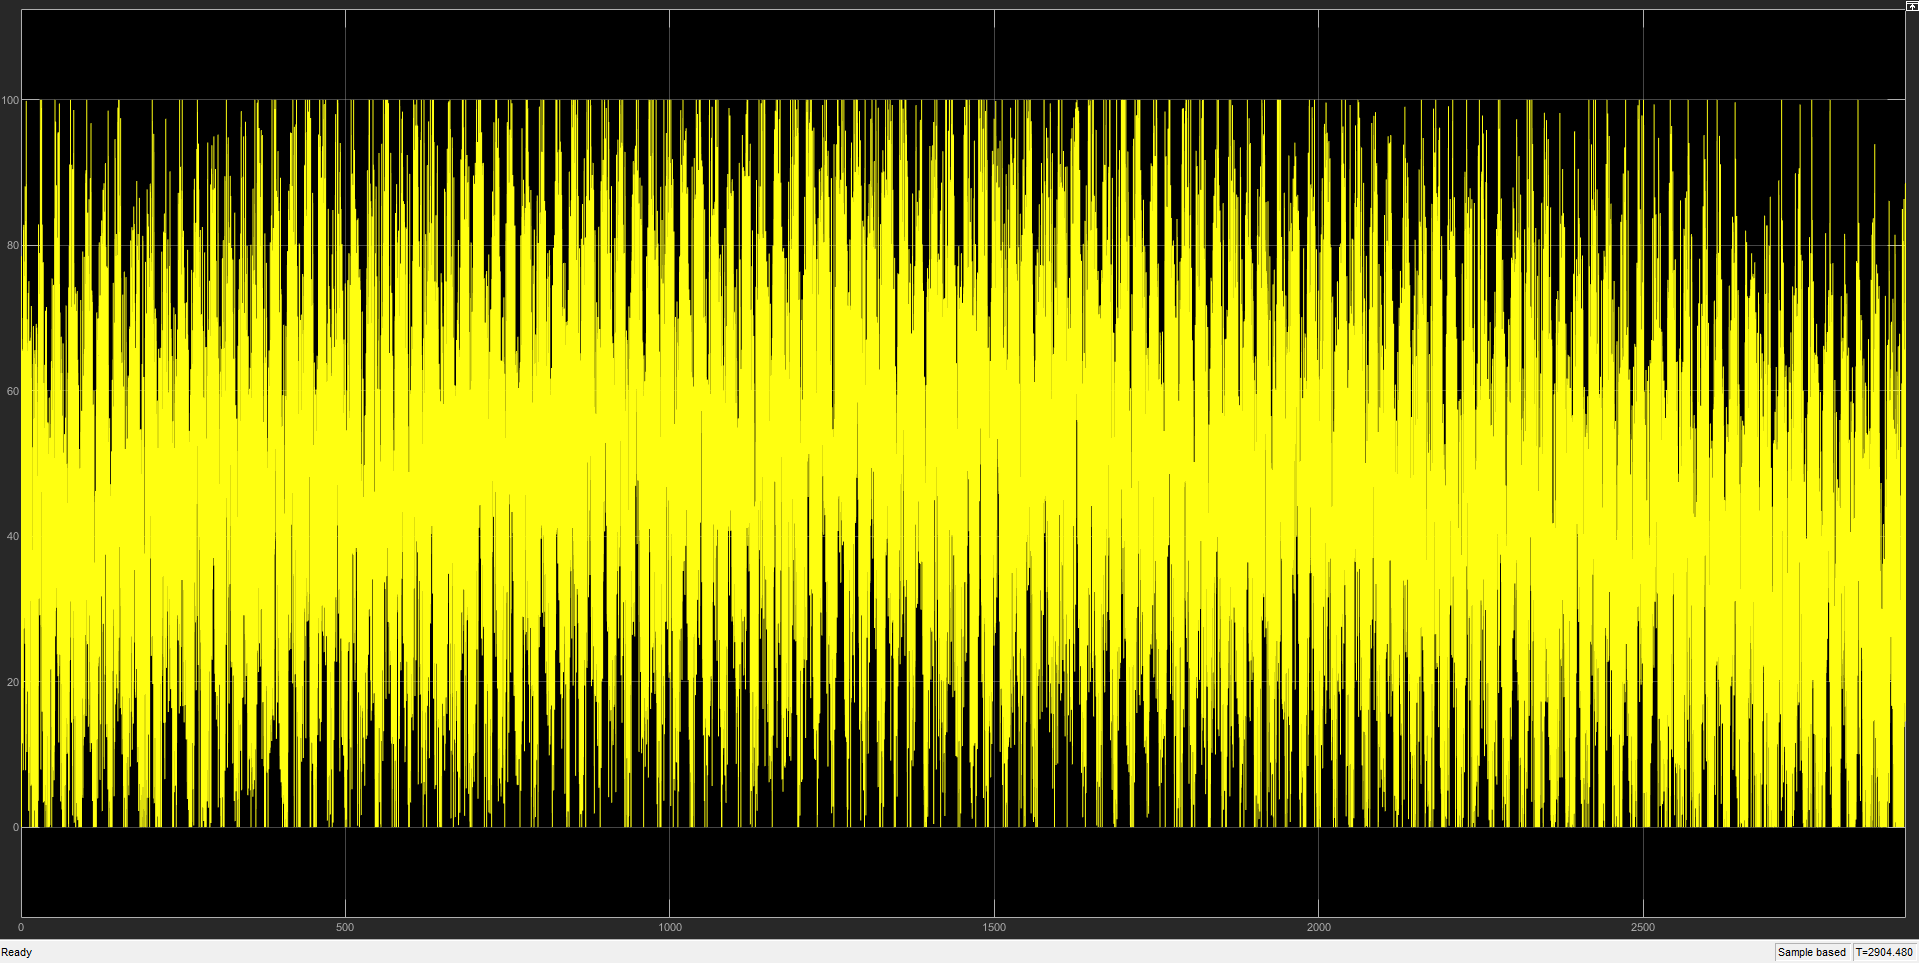
\includegraphics[height=0.9\textwidth,angle=90,origin=c]{images/sim_verlauf_feuchte.png}
    \caption[Simulierter Verlauf der rel. Feuchte]{Simulierter Verlauf der rel. Feuchte in \%H}
    \label{fi:sim_verlauf_feuchte}
    \end{figure}
    \subsection{Erzeugung der Datensätze}
    Die unterschiedlichen Datensätze werden durch 50 Simulationsdurchläufe erreicht (s. Abb. \ref{fi:sim_reihe}). Hierbei wird die Schleifenvariable $n$ als sog. Seed für die Zufallsgeneratoren in der Simulation genutzt, um die Reproduzierbarkeit der Ergebnisse sicherzustellen, während eine gewisse Varianz der Ergebnisse sichergestellt wird. Die jeweils generierten Verläufe werden in eine Excel Datei exportiert, wobei jeder Durchlauf in ein eigenes Blatt geschrieben wird. Der Hintergrund hierfür ist, dass Excel Dateien den quasi-Standard für den Import von Daten in die Software \ac{KNIME} darstellen.
    \begin{figure}[H]
        \begin{center}
            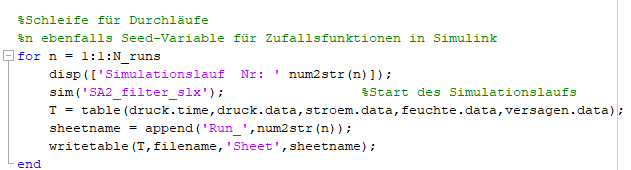
\includegraphics[width=\linewidth]{images/sim_reihe.png}
            \caption[M-file Simulationsreihen]{M-file: Abschnitt zur Erzeugung von Simulationsreihen und Export der Daten}
            \label{fi:sim_reihe}
        \end{center}
    \end{figure}
    \section{Analyse mit KNIME}
    \label{sec:knime}
    \ac{KNIME} ist eine freie Software zur interaktiven Datenanalyse. Die Software folgt dabei einem codeless-Ansatz über ein realtiv intuitiv bedienbares Interface, ermöglicht jedoch zusätzlich auch die Einbindung eigener Skripte in z.B. Python oder Java. Da KNIME unter der sog. GPL Lizenz vertrieben wird, ist die kommerzielle Nutzung freigestellt.
    Desweiteren stellt KNIME unterschiedliche Module zur Nutzung machinellen Lernens bereit. Nach Aufbereitung der Daten wurde hierbei zunächst ein sog. RProp MLP Learner verwendet (vgl. feedforward Netz Kap. \ref{sec:grundlagenKI}). Dieses Modell brachte allerdings keine zufriedenstellenden Ergebnisse, woraufhin ein \ac{DTL} Ansatz (REF) gewählt wurde. Um das Potenzial eines KI-basierten Ansatzes zu demonstrieren, wird das Modell mit den ersten 40 Simulationsdurchläufen trainiert, und anschließend auf die übrigen 10 Durchläufe angewendet. Die Ergebnisse bzw. die Bewertung der Genauigkeit der Vorhersage werden in Kapitel \ref{ch:schluss} vorgestellt. Die folgenden Unterkapitel erläutern den vollständigen Analyseprozesses in KNIME. \newline
    In Abb. \ref{fi:knime_all} ist die übergeordnete Struktur des KNIME Workflows zu sehen. Der Aufbau folgt dabei im wesentlichen den zahlreichen, auf der offiziellen Webseite vorgestellten, Beispielen \cite{knimehub}. Hierbei müssen zunächst die Daten importiert und vorbereitet werden, was hauptsächlich in der linken Metanode, am Start des Workflows, geschieht. Eine Metanode dient hierbei der Zusammenfassung von Unterkomponenten aus Gründen der Übersichtlichkeit. Anschließend werden die Daten in einen Datensatz zum Training des gewählten Vorhersagemodells (vgl. Decision Tree Learner in der Abb.), sowie in einen Datensatz zum Test (vgl. Decision Tree Predictor in der Abb.) des Modells geteilt. Im Anschluss werden die Testdaten, welche um die Vorhersage ergänzt wurden, an die Auswertung übergeben. Die Auswertung wurde in einer Metanode zusammengefasst.
    \begin{figure}[H]
        \begin{center}
            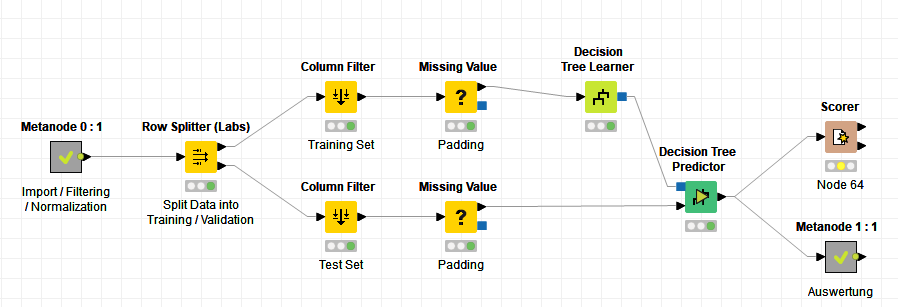
\includegraphics[width=\linewidth]{images/knime_all.png}
            \caption[KNIME Übersicht]{Übersicht des Workflows in KNIME}
            \label{fi:knime_all}
        \end{center}
    \end{figure}
    \subsection{Import und Transformation in KNIME}
    In der Import Metanode (s. Abb. \ref{fi:knime_import}) wird zunächst ein Excel Sheet eingelesen, welches die Namen der Arbeitsblätter, aber keine weiteren Daten enthält. Mit dieser Auflistung wird dann über Loop Nodes und der hiermit verschalteten, zweiten Excel Reader Node, die Excel Datei vollständig eingelesen, welche die Daten der Simulationsdurchläufe enthält. So wird die Beschränkung der Excel Reader Node umgangen, nur jeweils ein Arbeitsblatt einlesen zu können.
    In den Loop sind außerdem drei weitere Metanodes verkettet, welche der Datenaufbereitung dienen, und folgend erläutert werden.
    \begin{figure}[H]
        \begin{center}
            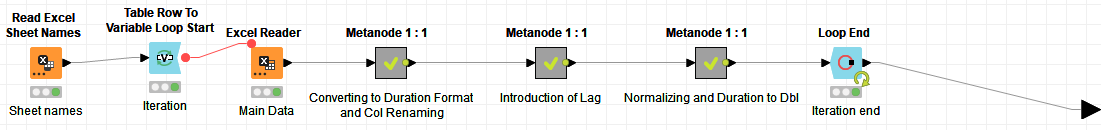
\includegraphics[width=\linewidth]{images/knime_import.png}
            \caption[KNIME Import Metanode]{Metanode zum Import und zur Vorbereitung der Daten in KNIME}
            \label{fi:knime_import}
        \end{center}
    \end{figure}
    Die ersten vier Nodes der ersten Metanode (s. Abb. \ref{fi:knime_filter}) dienen dazu, die Zeiteinheit der Simulationsdaten in ein von KNIME interpretierbares Format zu transformieren. 
    Anschließend werden die Spaltenüberschriften angepasst. Folgend werden die Zeilen der Datensätze, welche eine Strömungsgeschwindigkeit von 0 haben, aussortiert, und die Strömungsgeschwindigkeit-Spalte aggregiert, wobei die Strömungsgeschwindigkeit kummulativ behandelt wird. Das die Störmungsgeschwindigkeit kumulativ wirken muss, da sie in dieser Weise ein guter Indikator für die aufgenommene Staubmenge ist, kann als allgemeines Domänenwissen angesehen werden. Anschließend wird die Spalte für die Ist-Werte der Strömungsgeschwindigkeit, und alle Zeilen mit einem Differenzdruck kleiner \SI{800}{\pascal} fallen gelassen. 
    Der Wert wurde gewählt, weil als empfohlener Endwert \SI{600}{\pascal} im Datenblatt des Filters angegeben ist, wobei dieser lt. Datenblatt (s. Anhang) auch durchaus überschritten werden kann, weshalb der Bereich überhalb \SI{800}{\pascal} für die Analyse als lohnenswert zu sehen ist. Dies hat weiterhin den Vorteil, dass die Datenmenge die folgend verarbeitet werden muss, verringert wird, was die Durchlaufzeit weiterer Iterationschritte in der Entwicklung in KNIME verbessert hat.
    \begin{figure}[H]
        \begin{center}
            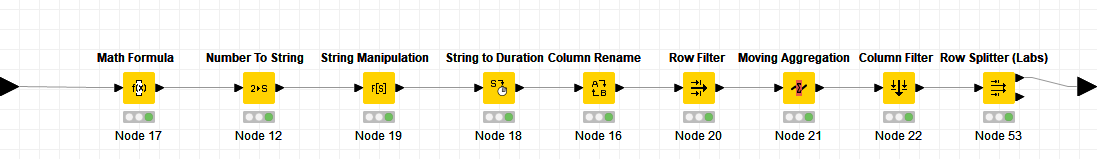
\includegraphics[width=\linewidth]{images/knime_filter.png}
            \caption[KNIME Filter Metanode]{Metanode zur ersten Aufbereitung und Filterung der Daten in KNIME}
            \label{fi:knime_filter}
        \end{center}
    \end{figure}
    In der zweiten Metanode der Import-Schleife (s. Abb. \ref{fi:knime_lag}) wird nun ein sog. Lag eingeführt. Lag meint hierbei die Verzögerung der Zustandsparameter  Strömungsgeschwindigkeit, Druckdifferenz und Feuchte. Das Ergebnis ist eine Datentabelle, in der eine Zeile die Werte der Zustandsparameter von vor einer Woche und die Werte für die Schadenswahrscheinlichkeit, sowie die vergangene Einsatzdauer enthält. Hierdurch wird ein Vorhersagehorizont von einer Woche angesetzt. Nach dem Deployment wäre ein perfektes Modell also in der Lage aus den jeweils aktuellen Werten eine Woche im voraus den Schadenswert vorherzusagen. Desweiteren werden die Werte für die Luftfeuchte geglättet, in dem ein gleitender Mittelwert aus den Feuchtewerten der jeweils letzten 24 Stunden gebildet wird. Hierdurch wird die tägliche Saisonalität der Feuchtewerte, und das Rauschen durch die Zufallsvariable in der Simulation (s. Abb. \ref{fi:sim_feuchteschwank}) kompensiert. Am Ende dieser Metanode werden außerdem in Folge der zeitlichen Verschiebung entstandene Zeilen mit nicht vorhandenen Werten aussortiert.
    \begin{figure}[H]
        \begin{center}
            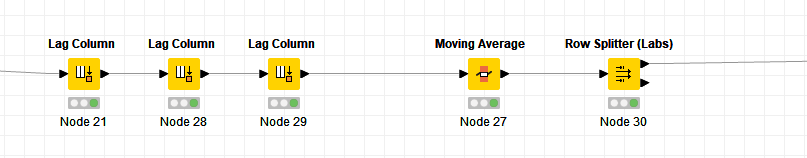
\includegraphics[width=\linewidth]{images/knime_lag.png}
            \caption[KNIME Lag Metanode]{Metanode zur Einführung von Lag in KNIME}
            \label{fi:knime_lag}
        \end{center}
    \end{figure}
    In der dritten Metanode der Import-Schleife (s. Abb. \ref{fi:knime_normal}) erfolgt nun die Normalisierung der Schadenswerte, bzw. die Transformation in eine Zeichenfolge, sowie die Vorgänge, die nötig sind um die Daten für die unterschiedlichen Modelle vorzubereiten. Die Abbildung zeigt hierbei den finalen Stand nach mehreren Iterationsschritten. Zunächst wird zunächst die \ac{KNIME} eigene Duration Variable wieder in Minuten als double zurücktransformiert. Auch wenn diese Variable später nicht bei der Klassifikation verwendet wird, wäre sie später ein guter Indikator für Alterungseffekte, welche allerdings von der Simulation in Simulink nicht abgedeckt werden. Dann werden die aktuellen Werte der Zustandsparameter fallen gelassen. Anschließend werden die Schadenswerte $>0 $ in FAIL und Werte $=0 $ in OK umgewandelt. Die Zahlenwerte repräsentieren zwar nur eine Wahrscheinlichkeit, aber um eine gewisse Sicherheit zu erreichen und um zunächst die Klassifikation durch ein \ac{DTL} zu erleichtern wird diese binäre Einteilung gewählt. Hierdurch wird diese in Klassen umgewandelt, die später vom \ac{DTL} Modell vorhergesagt werden können. Abschließend wird die Spalte mit den Schadenswahrscheinlichkeiten als Zahlenwert fallen gelassen. \\
    Diese Schleife wird nun von sämtlichen Datensätzen durchlaufen. Schlussendlich werden die  Durchläufe zu einer großen Datentabelle zusammengefügt, wobei die Tabelle um eine Spalte erweitert wird, welche die Iteration in der Schleife, bzw. die Durchlaufnummer darstellt. Hierfür wurde die Loop End Node (s. Abb. \ref{fi:knime_import}) verwendet. Es ist hervorzuheben, dass zwar der Lag und auch die Normalisierung in der Regel erst an späterer Stelle im Workflow in \ac{KNIME} durchgeführt wird. Dies würde allerdings dazu führen, dass auf Grund der Aneinanderreihung der Datensätze, beim Einführen der Verzögerung, die verganenen Werte des vorherigen Durchlaufs mit den Fehlerwahrscheinlichkeiten des folgenden Durchlaufs kombiniert werden würden. Deshalb müssen die Datensätze zunächst einzeln aufbereitet werden, bevor sie zusammengeführt werden.
    \begin{figure}[H]
        \begin{center}
            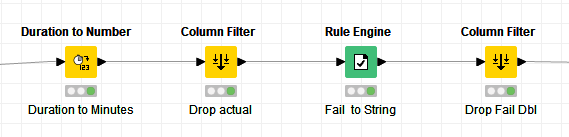
\includegraphics[width=\linewidth]{images/knime_normal.png}
            \caption[KNIME Normalizing Metanode]{Metanode zur Normalisierung der Schadenswerte in KNIME}
            \label{fi:knime_normal}
        \end{center}
    \end{figure}
    \subsection{Training und Test des DTL-Modells}
    Die Daten werden nun aufgeteilt in Trainins- und Testdaten. Hierzu wird der Datensatz anhand der eingeführten Variable zur Unterscheidung der Durchläufe getrennt. Die ersten 40 Durchläufe dienen dem Training des Modells, während die letzten 10 Durchläufe dem Test des Modells dienen (s. Abb. \ref{fi:knime_all}). Dies erfolgt in der der Row Splitter Node nach der Importschleife. Dann werden, im Falle der Trainingsdaten, die Spalten für Durchlaufnummer und Einsatzdauer fallen gelassen, und fehlende Werte durch Nullwerte ersetzt, um Fehlern vorzubeugen bzw. das Modell nicht mit irrelevanten Daten zu trainieren. Bei den Testdaten wird die Einsatzdauer beibehalten, da diese für die spätere Auswertung relevant ist.
    Die beiden Datensätze werden dann im \ac{KNIME} typischen Learner/Predictor Schema verarbeitet. Der Learner trainiert hierbei das Modell, und gibt es am Ausgang aus (s. Abb. \ref{fi:knime_dtl}). Der Predictor erhält das mit den Trainingsdaten angelernte Modell und wendet es auf die Testdaten an, wobei die Datentabelle um eine Spalte mit der Vorhersage erweitert wird (s. Abb. \ref{fi:knime_table}). An den Spaltenüberschriften ist die Verzögerung von $16800 \frac{h}{100} = 168 h = 7 d $ zu erkennen.  \\
    \begin{figure}[H]
        \begin{center}
            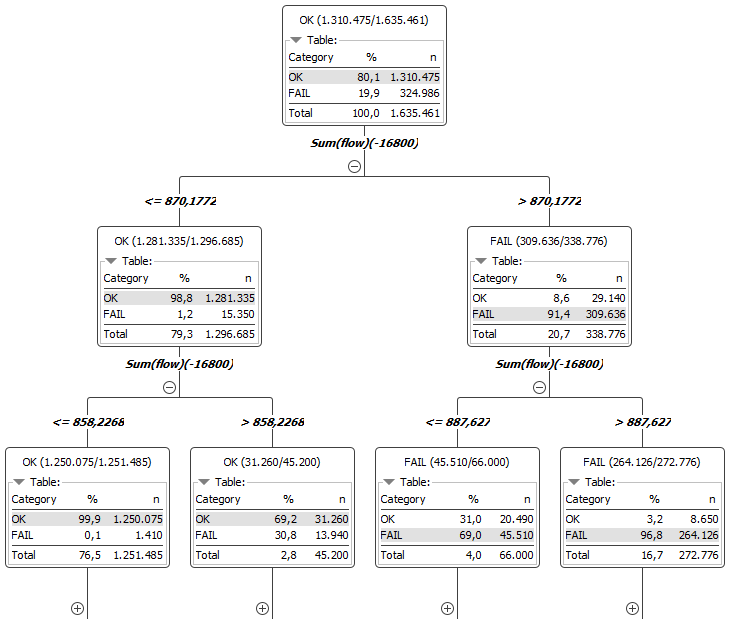
\includegraphics[width=\linewidth]{images/knime_dtl.png}
            \caption[KNIME DTL Baum]{Baumansicht der ersten zwei Splits des DTL Modells in KNIME}
            \label{fi:knime_dtl}
        \end{center}
    \end{figure}
    \begin{figure}[H]
        \begin{center}
            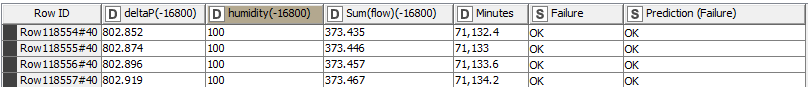
\includegraphics[width=\linewidth]{images/knime_table.png}
            \caption[KNIME Vorhersagetabelle]{Tabellenansicht der Daten nach der Vorhersage durch das trainierte DTL Modell}
            \label{fi:knime_table}
        \end{center}
    \end{figure}
    \subsection{Auswertung in KNIME}
    \label{sec:knime_auswertung}
    Die Bewertung der Vorhersagequalität erfolgte zunächst mit der von KNIME bereitgestellten Scorer Node (s. Abb. \ref{fig:wertungen}). Diese Wertungen wurden genutzt, um die Parameter des \ac{DTL} Modells (s. Kap \ref{sec:dtl}), sowie die vorherige Datentransformation und -normalisierung zu variieren, und somit empirisch eine gute Kombination zu ermitteln. Die Screenshots zeigen hierbei sowohl die ungefilterte Wertung, als auch eine Wertung, bei der vorhergehend die Kombination OK/OK von Vorhersage und simulierten Schadenswert aussortiert wurde. 
    Die ungefilterte Wertung zeigt hierbei ein Cohens Kappa, ein statistisches Maß für die Übereinstimmung von zwei sog. Beobachtern, von $\kappa  = 0,881$, was in der Literatur allgemein als ausgzeichneter Wert gilt. Die ungefilterte Wertung zeigt eine Übereinstimmung von 82\%, was ebenfalls als ausreichend genau bewertet wurde, da diese Metrik im Kontext des betrachteten Zeitraums gesehen werden muss, worauf in Kap. \ref{sec:ergebnisse} näher eingegangen wird. Von insgesamt 414300 (entspricht 4143 h)  betrachteten Zeilen (s. \ref{fi:knime_score1}) wertete das Modell nur 3522 (entspricht 35,2 h) fehlerhaft als Schaden (FAIL) und nur 10902 (entspricht 109 h)  fehlerhaft als funktional (OK) bei 10 analysierten Durchläufen.
    Die in Abb. \ref{fi:knime_all} am Ende des Workflows implementierte Metanode umfasst die automatisierte Auswertung der Ergebnisse im Kontext der Vorhersagezeit (s. Kap. \ref{sec:ergebnisse}). 
    \begin{figure}[H]
        \begin{center}
    %
           \subfigure[Wertung (Score) der Vorhersage in KNIME]{%
               \label{fi:knime_score1}
               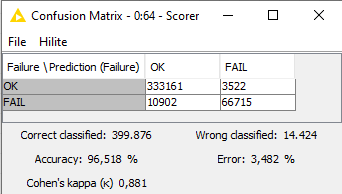
\includegraphics[width=0.5\textwidth]{images/knime_score1.png}
           }%
           \subfigure[Wertung (Score) der Vorhersage in KNIME ohne den Fall OK/OK]{%
              \label{fi:knime_score2}
              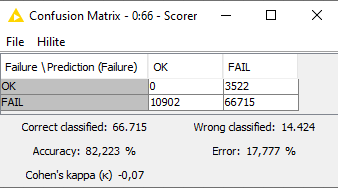
\includegraphics[width=0.5\textwidth]{images/knime_score2.png}
           }\\ %  ------- End of the first row ----------------------%
    %
       \end{center}
       \caption{%
           Wertung (Score) und gefilterte Wertung der Vorhersage durch Scorer Nodes in KNIME
        }%
      \label{fig:wertungen}
    \end{figure}
